% !TeX program = xelatex
\documentclass[a4paper,10pt]{article}

% ============================================================================
% កញ្ចប់បណ្ណាល័យ (Packages) – តាមលំនាំស្តង់ដារអនុវិទ្យាល័យព្រះក្រសាំង (ls_plan.tex)
% ============================================================================
\usepackage[a4paper, left=0.95cm, right=0.95cm, top=0.85cm, bottom=0.92cm, footskip=0.52cm]{geometry}
\usepackage{amsmath}
\usepackage{unicode-math}
\usepackage{fontspec}
\usepackage{array, longtable, multirow, colortbl}
\usepackage[table]{xcolor}
\usepackage{enumitem}
\usepackage{pifont}
\usepackage{fancyhdr}
\usepackage{tikz}
\usetikzlibrary{calc, arrows.meta, angles, quotes, decorations.markings, babel}

% LaTeX 2025 + longtable compatibility guard
\makeatletter
\let\@expl@@@mark@update@singlecol@structures@@\relax
\makeatother

% ============================================================================
% ការកំណត់ពុម្ពអក្សរ (Cross-Platform Windows + Linux Cloud fonts/)
% ============================================================================
\providecommand{\NGSFindFonts}{%
  \IfFileExists{C:/Windows/Fonts/cambria.ttc}{%
    \def\NGSSysPath{C:/Windows/Fonts/}%
    \def\NGSUserPath{C:/Users/KIT/AppData/Local/Microsoft/Windows/Fonts/}%
  }{%
    \IfFileExists{./fonts/KhmerOSsiemreap.ttf}{\def\NGSSysPath{./fonts/}\def\NGSUserPath{./fonts/}}{%
    \IfFileExists{../fonts/KhmerOSsiemreap.ttf}{\def\NGSSysPath{../fonts/}\def\NGSUserPath{../fonts/}}{%
    \IfFileExists{../../fonts/KhmerOSsiemreap.ttf}{\def\NGSSysPath{../../fonts/}\def\NGSUserPath{../../fonts/}}{%
    \IfFileExists{../../../fonts/KhmerOSsiemreap.ttf}{\def\NGSSysPath{../../../fonts/}\def\NGSUserPath{../../../fonts/}}{%
    \IfFileExists{../../../../fonts/KhmerOSsiemreap.ttf}{\def\NGSSysPath{../../../../fonts/}\def\NGSUserPath{../../../../fonts/}}{%
    \IfFileExists{../../../../../fonts/KhmerOSsiemreap.ttf}{\def\NGSSysPath{../../../../../fonts/}\def\NGSUserPath{../../../../../fonts/}}{%
    \IfFileExists{../../../../../../fonts/KhmerOSsiemreap.ttf}{\def\NGSSysPath{../../../../../../fonts/}\def\NGSUserPath{../../../../../../fonts/}}{%
      \def\NGSSysPath{../../../../../../../fonts/}\def\NGSUserPath{../../../../../../../fonts/}%
    }}}}}}}%
  }%
}
\NGSFindFonts

\setmathfont[
  Path={\NGSSysPath},
  FontIndex=1,
  Scale=1.02
]{cambria.ttc}

\defaultfontfeatures{Ligatures=TeX}

\setmainfont[
  Path={\NGSUserPath},
  Extension=.ttf,
  Script=Khmer,
  BoldFont={KhmerOSsiemreap},
  BoldFeatures={FakeBold=1.8},
  ItalicFont={KhmerOSsiemreap},
  ItalicFeatures={FakeSlant=0.25},
  BoldItalicFont={KhmerOSsiemreap},
  BoldItalicFeatures={FakeBold=1.8, FakeSlant=0.25}
]{KhmerOSsiemreap}

\newfontfamily\muol[
  Path={\NGSUserPath},
  Extension=.ttf,
  Script=Khmer
]{KhmerOSmuollight}

\newfontfamily\TimesEn[
  Path={\NGSSysPath},
  Extension=.ttf,
  Scale=1.00,
  BoldFont={timesbd},
  ItalicFont={timesi},
  BoldItalicFont={timesbi}
]{times}

\newfontfamily\NagaBold[
  Path={\NGSUserPath},
  Extension=.ttf
]{AKbalthom Naga Bold}

\newfontfamily\CalibriFont[
  Path={\NGSSysPath},
  Extension=.ttf
]{calibri}

\newfontfamily\Tacteing[
  Path={\NGSUserPath}
]{TACTENG.TTF}

\newfontfamily\CourierBullet[
  Path={\NGSSysPath},
  Extension=.ttf
]{cour}
\newcommand{\wcirc}{{\CourierBullet\fontsize{9.5pt}{11pt}\selectfont o}}

\XeTeXlinebreaklocale "km"
\XeTeXlinebreakskip = 0pt plus 1pt minus 0.1pt

% ============================================================================
% ពណ៌ និងទម្រង់ទំព័រ
% ============================================================================
\definecolor{stepgray}{HTML}{D9D9D9}
\definecolor{headgray}{HTML}{F2F2F2}
\definecolor{boxgray}{HTML}{E6E6E6}
\definecolor{darkred}{HTML}{C00000}
\definecolor{red5e}{HTML}{FF0000}

\pagestyle{fancy}
\fancyhf{}
\renewcommand{\headrulewidth}{0pt}
\fancyfoot[R]{\CalibriFont\fontsize{11pt}{13pt}\selectfont\thepage}

\setlength{\parindent}{0pt}
\setlength{\parskip}{0pt}
\setlength{\tabcolsep}{3.8pt}

\newcolumntype{L}[1]{>{\raggedright\arraybackslash}p{#1}}
\newcolumntype{C}[1]{>{\centering\arraybackslash}p{#1}}

% ============================================================================
% ម៉ាក្រូជំនួយ (Helper Macros)
% ============================================================================
\newcommand{\en}[1]{{\TimesEn #1}}
\newcommand{\enbf}[1]{{\TimesEn\textbf{#1}}}
\newcommand{\unit}[1]{\,\text{\en{#1}}}
\newcommand{\fiveE}[1]{{\NagaBold\fontsize{9.5pt}{13pt}\selectfont\textcolor{red5e}{#1}}}
\newcommand{\timenote}[1]{\textcolor{darkred}{\textit{#1}}}
\newcommand{\graybox}[1]{\colorbox{boxgray}{\strut\hspace{2pt}#1\hspace{2pt}}}
\newcommand{\ditem}{\tikz[baseline=-0.5ex]\fill (0,0.42ex) -- (0.42ex,0) -- (0,-0.42ex) -- (-0.42ex,0) -- cycle;\hspace{0.3em}}
\newcommand{\cnum}[1]{{\fontsize{10.5pt}{12pt}\selectfont\ding{\numexpr181+#1\relax}}\hspace{0.2em}}
\newcommand{\cfig}[1]{\par\vspace{4pt}{\centering #1\par}\vspace{4pt}}
\newcommand{\stepheader}[1]{\multicolumn{3}{|c|}{\cellcolor{stepgray}\muol #1} \\* \noalign{\hrule height 0.4pt}}
\newcommand{\tri}[1]{\ensuremath{\triangle #1}}
\newcommand{\ang}[1]{\ensuremath{\angle #1}}
\newcommand{\cg}{\ensuremath{\cong}}
\newcommand{\chkbox}{\tikz[baseline=-0.15ex]\draw[black, line width=0.8pt] (0,0) rectangle (0.23cm,0.23cm);}

\tikzset{
  tk1/.style={postaction={decorate},decoration={markings,mark=at position 0.50 with {\draw[black, line width=0.85pt](0,-0.095)--(0,0.095);}}},
  tk2/.style={postaction={decorate},decoration={markings,
    mark=at position 0.45 with {\draw[black, line width=0.85pt](0,-0.095)--(0,0.095);},
    mark=at position 0.55 with {\draw[black, line width=0.85pt](0,-0.095)--(0,0.095);}}}
}

\newcommand{\rightbox}[4][0.18]{%
  \draw[black, line width=0.8pt]
    ($(#3)!#1!(#2)$) -- ($($(#3)!#1!(#2)$)+($(#3)!#1!(#4)$)-(#3)$) -- ($(#3)!#1!(#4)$);
}

\newcommand{\khmflourish}{{\Tacteing\fontsize{36pt}{14pt}\selectfont\raisebox{-5pt}{3}}}

% ============================================================================
% ម៉ាក្រូគូសរូបធរណីមាត្រ B&W ច្បាស់សមាមាត្រ (3.8–6.8 cm, អក្សរខ្មៅ 100%)
% ============================================================================

% ១. រំលឹកមេរៀនចាស់៖ មុំក្រៅនៃត្រីកោណ និងកន្លះបន្ទាត់ពុះមុំក្រៅកែងនឹងកន្លះបន្ទាត់ពុះមុំក្នុង
\newcommand{\figPrereqEXB}{%
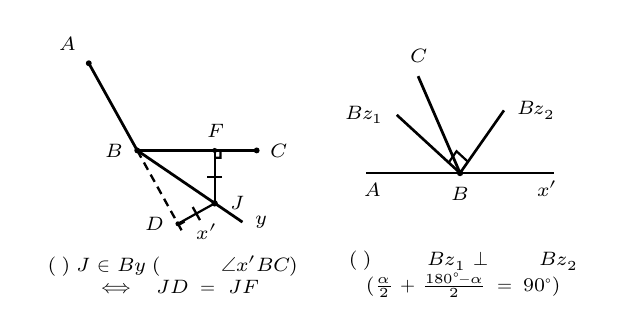
\begin{tikzpicture}[scale=0.82, every node/.style={font=\scriptsize, text=black}]
  % (១) កន្លះបន្ទាត់ពុះមុំក្រៅ By ស្មើចម្ងាយពី BC និងបន្ទាត់បន្លាយ ABx'
  \begin{scope}[shift={(0,0)}]
    \coordinate (A) at (-1.10,1.25);
    \coordinate (B) at (-0.35,-0.10);
    \coordinate (C) at (1.50,-0.10);
    \coordinate (Xp) at (0.35,-1.36);
    \coordinate (J) at (0.85,-0.92);
    \coordinate (F) at (0.85,-0.10);
    \coordinate (D) at ($(A)!(J)!(Xp)$);
    \draw[black, line width=1.0pt] (A) -- (B) -- (C);
    \draw[black, line width=0.85pt, densely dashed] (B) -- (Xp) node[right=1.5pt] {$x'$};
    \draw[black, line width=1.0pt] (B) -- (1.28,-1.21) node[right=1pt] {$y$};
    \draw[black, line width=0.8pt, tk1] (J) -- (F);
    \draw[black, line width=0.8pt, tk1] (J) -- (D);
    \rightbox[0.14]{J}{F}{C}
    \rightbox[0.14]{J}{D}{Xp}
    \fill[black] (A) circle (1.3pt) node[above left=1pt] {$A$};
    \fill[black] (B) circle (1.3pt) node[left=2pt] {$B$};
    \fill[black] (C) circle (1.3pt) node[right=1.5pt] {$C$};
    \fill[black] (J) circle (1.4pt) node[right=2pt] {$J$};
    \fill[black] (F) circle (1.1pt) node[above=1pt] {$F$};
    \fill[black] (D) circle (1.1pt) node[left=1.5pt] {$D$};
    \node[align=center, text width=3.45cm] at (0.20,-2.02) {(១) $J\in By$ (ពុះមុំក្រៅ $\ang{x'BC}$)\\$\iff JD = JF$};
  \end{scope}

  % (២) កន្លះបន្ទាត់ពុះមុំក្នុង និងកន្លះបន្ទាត់ពុះមុំក្រៅកែងគ្នា (90°)
  \begin{scope}[shift={(4.65,0)}]
    \coordinate (X1) at (-1.45,-0.45);
    \coordinate (B) at (0,-0.45);
    \coordinate (X2) at (1.45,-0.45);
    \coordinate (C) at (-0.65,1.05);
    \coordinate (Bi) at (-0.98,0.45);
    \coordinate (Be) at (0.68,0.52);
    \draw[black, line width=1.0pt] (X1) -- (X2);
    \draw[black, line width=1.0pt] (B) -- (C) node[above=1pt] {$C$};
    \draw[black, line width=0.95pt] (B) -- (Bi) node[left=1pt] {$Bz_1$};
    \draw[black, line width=0.95pt] (B) -- (Be) node[right=1pt] {$Bz_2$};
    \rightbox[0.18]{Bi}{B}{Be}
    \fill[black] (B) circle (1.4pt) node[below=1.5pt] {$B$};
    \node at (-1.35,-0.70) {$A$};
    \node at (1.35,-0.70) {$x'$};
    \node[align=center, text width=3.45cm] at (0.05,-2.02) {(២) ពុះក្នុង $Bz_1 \perp$ ពុះក្រៅ $Bz_2$\\($\frac{\alpha}{2}+\frac{180^\circ-\alpha}{2}=90^\circ$)};
  \end{scope}
\end{tikzpicture}}

% ២. E1 Engage: ប៉មភ្លើងសញ្ញាសុវត្ថិភាព J នៅក្រៅផ្លូវបំបែកត្រីកោណ ABC ប៉ុន្តែស្មើចម្ងាយពីផ្លូវត្រង់ទាំងបី
\newcommand{\figEngageEXB}{%
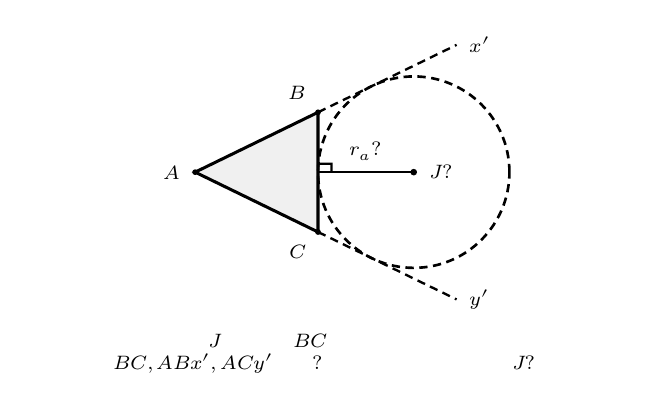
\begin{tikzpicture}[scale=0.80, every node/.style={font=\scriptsize, text=black}]
  \coordinate (A) at (-1.80,0);
  \coordinate (B) at (0.15,0.95);
  \coordinate (C) at (0.15,-0.95);
  \coordinate (X1) at (2.35,2.02);
  \coordinate (X2) at (2.35,-2.02);
  \pgfmathsetmacro{\lc}{veclen(1.95,0.95)}
  \pgfmathsetmacro{\lb}{\lc}
  \pgfmathsetmacro{\la}{1.90}
  \pgfmathsetmacro{\den}{\lb+\lc-\la}
  \pgfmathsetmacro{\jx}{(-\la*(-1.80)+\lb*0.15+\lc*0.15)/\den}
  \coordinate (J) at (\jx,0);
  \pgfmathsetmacro{\rj}{\jx-0.15}
  \fill[gray!12] (A) -- (B) -- (C) -- cycle;
  \draw[black, line width=1.1pt] (A) -- (B) -- (C) -- cycle;
  \draw[black, line width=0.85pt, densely dashed] (B) -- (X1) node[right=1pt] {$x'$};
  \draw[black, line width=0.85pt, densely dashed] (C) -- (X2) node[right=1pt] {$y'$};
  \draw[black, line width=0.95pt, densely dashed] (J) circle (\rj cm);
  \coordinate (Fa) at (0.15,0);
  \draw[black, line width=0.8pt] (J) -- (Fa) node[midway, above=0.5pt] {$r_a?$};
  \rightbox[0.14]{J}{Fa}{B}
  \fill[black] (A) circle (1.3pt) node[left=2pt] {$A$};
  \fill[black] (B) circle (1.3pt) node[above left=1pt] {$B$};
  \fill[black] (C) circle (1.3pt) node[below left=1pt] {$C$};
  \fill[black] (J) circle (1.5pt) node[right=2pt] {$J?$};
  \node[align=center, text width=7.3cm] at (0.25,-2.88) {តើមានចំណុច $J$ នៅក្រៅជ្រុង $BC$ ដែលស្មើចម្ងាយពីផ្លូវត្រង់ទាំងបី $BC, ABx', ACy'$ ដែរឬទេ? តើកន្លះបន្ទាត់ណាខ្លះជួបគ្នាត្រង់ $J$?};
\end{tikzpicture}}

% ៣. E2/E3 ឧទាហរណ៍ និងទ្រឹស្តីបទផ្ចិតរង្វង់ចារឹកក្នុងមុំក្រៅត្រីកោណ (ទំ.២១១–២១២៖ រង្វង់ផ្ចិត J ប៉ះ D, E, F)
\newcommand{\figExcenterProof}{%
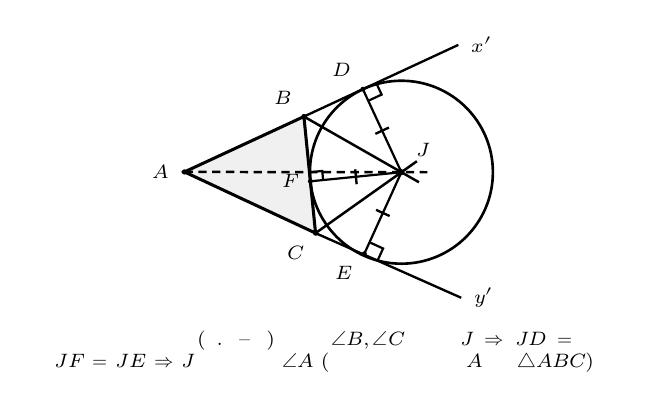
\begin{tikzpicture}[scale=0.74, every node/.style={font=\scriptsize, text=black}]
  \coordinate (A) at (-2.30,0.10);
  \coordinate (B) at (-0.25,1.05);
  \coordinate (C) at (-0.05,-0.95);
  \coordinate (Bx) at (2.40,2.28);
  \coordinate (Cy) at (2.45,-2.06);
  \pgfmathsetmacro{\la}{veclen(0.20,-2.00)}
  \pgfmathsetmacro{\lb}{veclen(2.25,-1.05)}
  \pgfmathsetmacro{\lc}{veclen(2.05,0.95)}
  \pgfmathsetmacro{\den}{\lb+\lc-\la}
  \pgfmathsetmacro{\jx}{(-\la*(-2.30)+\lb*(-0.25)+\lc*(-0.05))/\den}
  \pgfmathsetmacro{\jy}{(-\la*(0.10)+\lb*(1.05)+\lc*(-0.95))/\den}
  \coordinate (J) at (\jx,\jy);
  \coordinate (F) at ($(B)!(J)!(C)$);
  \coordinate (D) at ($(A)!(J)!(Bx)$);
  \coordinate (E) at ($(A)!(J)!(Cy)$);

  \fill[gray!12] (A) -- (B) -- (C) -- cycle;
  \draw[black, line width=1.1pt] (A) -- (B) -- (C) -- cycle;
  \draw[black, line width=0.85pt] (B) -- (Bx) node[right=1pt] {$x'$};
  \draw[black, line width=0.85pt] (C) -- (Cy) node[right=1pt] {$y'$};

  % ប្រើ through / calc សម្រាប់កាំរង្វង់ចារឹកក្នុងមុំក្រៅ J
  \path let \p1 = ($(J)-(F)$), \n1 = {veclen(\x1,\y1)} in
    \pgfextra{\xdef\radJ{\n1}};
  \draw[black, line width=0.95pt] (J) circle (\radJ);

  \draw[black, line width=0.9pt] (B) -- ($(B)!1.18!(J)$);
  \draw[black, line width=0.9pt] (C) -- ($(C)!1.18!(J)$);
  \draw[black, line width=0.9pt, densely dashed] (A) -- ($(A)!1.12!(J)$);

  \draw[black, line width=0.8pt, tk1] (J) -- (D);
  \draw[black, line width=0.8pt, tk1] (J) -- (E);
  \draw[black, line width=0.8pt, tk1] (J) -- (F);
  \rightbox[0.14]{J}{D}{Bx}
  \rightbox[0.14]{J}{E}{Cy}
  \rightbox[0.14]{J}{F}{B}

  \fill[black] (A) circle (1.3pt) node[left=2pt] {$A$};
  \fill[black] (B) circle (1.3pt) node[above left=1pt] {$B$};
  \fill[black] (C) circle (1.3pt) node[below left=1pt] {$C$};
  \fill[black] (J) circle (1.5pt) node[above right=2pt] {$J$};
  \fill[black] (D) circle (1.2pt) node[above left=1pt] {$D$};
  \fill[black] (E) circle (1.2pt) node[below left=1pt] {$E$};
  \fill[black] (F) circle (1.2pt) node[left=1.5pt] {$F$};
  \node[align=center, text width=7.3cm] at (0.10,-2.98) {ឧទាហរណ៍ និងទ្រឹស្តីបទ (ទំ.២១១--២១២)៖ ពុះក្រៅ $\ang{B},\ang{C}$ ជួបត្រង់ $J \Rightarrow JD=JF=JE \Rightarrow J$ នៅលើពុះក្នុងនៃ $\ang{A}$ (ផ្ចិតរង្វង់ចារឹកក្នុងមុំ $A$ ក្រៅ $\tri{ABC}$)};
\end{tikzpicture}}

% ៤. E4 ការគណនាមុំត្រង់ផ្ចិត I, J និង លំហាត់ទី៨ (ទំ.២១៣៖ AP = PQ = QC = AC/3)
\newcommand{\figElaborateEXB}{%
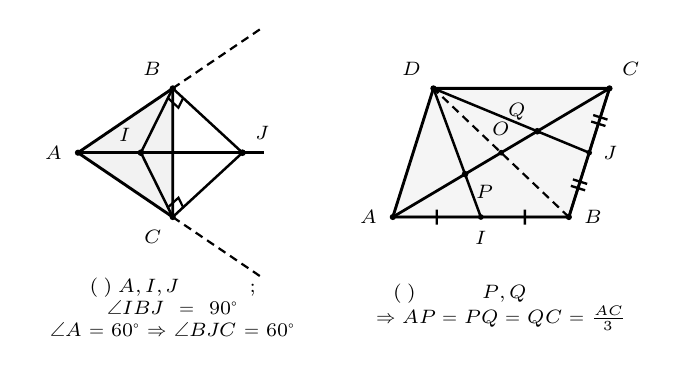
\begin{tikzpicture}[scale=0.86, every node/.style={font=\scriptsize, text=black}]
  % (ក) ទំនាក់ទំនង A, I, J រត់ត្រង់ជួរគ្នា និង ∠IBJ = ∠ICJ = 90°
  \begin{scope}[shift={(0,0)}]
    \coordinate (A) at (-1.55,0);
    \coordinate (B) at (-0.15,0.95);
    \coordinate (C) at (-0.15,-0.95);
    \coordinate (I) at (-0.62,0);
    \coordinate (J) at (0.88,0);
    \fill[gray!10] (A) -- (B) -- (C) -- cycle;
    \draw[black, line width=1.05pt] (A) -- (B) -- (C) -- cycle;
    \draw[black, line width=0.8pt, densely dashed] (B) -- (1.15,1.83);
    \draw[black, line width=0.8pt, densely dashed] (C) -- (1.15,-1.83);
    \draw[black, line width=0.9pt] (A) -- (1.20,0);
    \draw[black, line width=0.9pt] (B) -- (I) -- (C) -- (J) -- (B);
    \rightbox[0.15]{I}{B}{J}
    \rightbox[0.15]{I}{C}{J}
    \fill[black] (A) circle (1.3pt) node[left=2pt] {$A$};
    \fill[black] (B) circle (1.3pt) node[above left=1pt] {$B$};
    \fill[black] (C) circle (1.3pt) node[below left=1pt] {$C$};
    \fill[black] (I) circle (1.4pt) node[above left=0.5pt] {$I$};
    \fill[black] (J) circle (1.4pt) node[above right=1pt] {$J$};
    \node[align=center, text width=3.45cm] at (-0.15,-2.28) {(ក) $A, I, J$ ត្រង់ជួរគ្នា; $\ang{IBJ}=90^\circ$\\$\ang{A}=60^\circ \Rightarrow \ang{BJC}=60^\circ$};
  \end{scope}

  % (ខ) លំហាត់ទី៨ (ទំ.២១៣)៖ ប្រលេឡូក្រាម ABCD, AP = PQ = QC = AC/3
  \begin{scope}[shift={(4.65,0)}]
    \coordinate (A) at (-1.55,-0.95);
    \coordinate (B) at (1.05,-0.95);
    \coordinate (C) at (1.65,0.95);
    \coordinate (D) at (-0.95,0.95);
    \coordinate (I) at ($0.5*(A)+0.5*(B)$);
    \coordinate (J) at ($0.5*(B)+0.5*(C)$);
    \coordinate (O) at ($0.5*(A)+0.5*(C)$);
    \coordinate (P) at ($0.6667*(O)+0.3333*(A)$);
    \coordinate (Q) at ($0.6667*(O)+0.3333*(C)$);
    \fill[gray!8] (A) -- (B) -- (C) -- (D) -- cycle;
    \draw[black, line width=1.05pt] (A) -- (B) -- (C) -- (D) -- cycle;
    \draw[black, line width=1.0pt] (A) -- (C);
    \draw[black, line width=0.8pt, densely dashed] (B) -- (D);
    \draw[black, line width=0.9pt] (D) -- (I) (D) -- (J);
    \draw[black, line width=0.8pt, tk1] (A) -- (I);
    \draw[black, line width=0.8pt, tk1] (I) -- (B);
    \draw[black, line width=0.8pt, tk2] (B) -- (J);
    \draw[black, line width=0.8pt, tk2] (J) -- (C);
    \fill[black] (A) circle (1.3pt) node[left=2pt] {$A$};
    \fill[black] (B) circle (1.3pt) node[right=2pt] {$B$};
    \fill[black] (C) circle (1.3pt) node[above right=1pt] {$C$};
    \fill[black] (D) circle (1.3pt) node[above left=1pt] {$D$};
    \fill[black] (I) circle (1.2pt) node[below=1.5pt] {$I$};
    \fill[black] (J) circle (1.2pt) node[right=1.5pt] {$J$};
    \fill[black] (O) circle (1.2pt) node[above=2.5pt] {$O$};
    \fill[black] (P) circle (1.4pt) node[below right=0.5pt] {$P$};
    \fill[black] (Q) circle (1.4pt) node[above left=0.5pt] {$Q$};
    \node[align=center, text width=3.45cm] at (0.05,-2.28) {(ខ) លំហាត់ទី៨៖ $P, Q$ ទីប្រជុំទម្ងន់\\$\Rightarrow AP = PQ = QC = \frac{AC}{3}$};
  \end{scope}
\end{tikzpicture}}

% ៥. កំណែកិច្ចការផ្ទះទី១២ (ទំ.២១៤) និងតម្រុយលំហាត់ទី១១ (ទំ.២១៤៖ O កណ្ដាល HH')
\newcommand{\figHWReviewEXB}{%
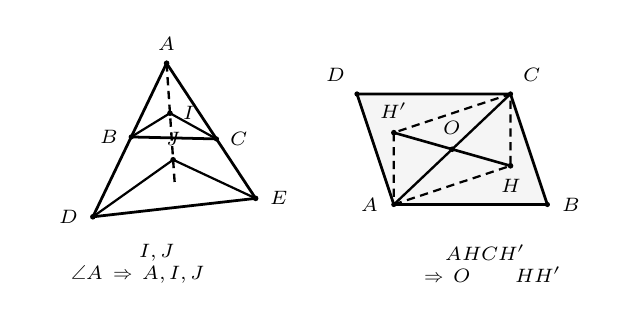
\begin{tikzpicture}[scale=0.78, every node/.style={font=\scriptsize, text=black}]
  % (ក) លំហាត់ទី១២ (ទំ.២១៤)
  \begin{scope}[shift={(0,0)}]
    \coordinate (A) at (0,1.45);
    \coordinate (D) at (-1.20,-1.05);
    \coordinate (E) at (1.45,-0.75);
    \coordinate (B) at ($(A)!0.48!(D)$);
    \coordinate (C) at ($(A)!0.56!(E)$);
    \pgfmathsetmacro{\ab}{veclen(-0.576,-1.20)}
    \pgfmathsetmacro{\ac}{veclen(0.812,-1.232)}
    \pgfmathsetmacro{\bc}{veclen(1.388,-0.032)}
    \pgfmathsetmacro{\pabc}{\ab+\ac+\bc}
    \coordinate (I) at ({(\ab*0.812+\ac*(-0.576))/\pabc}, {1.45+(\ab*(-1.232)+\ac*(-1.20))/\pabc});
    \pgfmathsetmacro{\ad}{veclen(-1.20,-2.50)}
    \pgfmathsetmacro{\ae}{veclen(1.45,-2.20)}
    \pgfmathsetmacro{\de}{veclen(2.65,0.30)}
    \pgfmathsetmacro{\pade}{\ad+\ae+\de}
    \coordinate (J) at ({(\ad*1.45+\ae*(-1.20))/\pade}, {1.45+(\ad*(-2.20)+\ae*(-2.50))/\pade});
    \draw[black, line width=1.0pt] (A) -- (D) -- (E) -- cycle;
    \draw[black, line width=1.0pt] (B) -- (C);
    \draw[black, line width=0.8pt] (B) -- (I) -- (C) (D) -- (J) -- (E);
    \draw[black, line width=0.85pt, densely dashed] (A) -- ($(A)!1.25!(J)$);
    \fill[black] (A) circle (1.3pt) node[above=1pt] {$A$};
    \fill[black] (B) circle (1.2pt) node[left=1.5pt] {$B$};
    \fill[black] (C) circle (1.2pt) node[right=1.5pt] {$C$};
    \fill[black] (D) circle (1.3pt) node[left=2pt] {$D$};
    \fill[black] (E) circle (1.3pt) node[right=2pt] {$E$};
    \fill[black] (I) circle (1.3pt) node[right=1.5pt] {$I$};
    \fill[black] (J) circle (1.3pt) node[above=1.5pt] {$J$};
    \node[align=center, text width=3.45cm] at (0.10,-1.82) {លំហាត់ទី១២៖ $I, J$ នៅលើពុះក្នុងរួមនៃ $\ang{A} \Rightarrow A, I, J$ ត្រង់ជួរគ្នា};
  \end{scope}

  % (ខ) តម្រុយលំហាត់ទី១១ (ទំ.២១៤៖ O ចំណុចកណ្ដាល HH')
  \begin{scope}[shift={(4.65,0)}]
    \coordinate (A2) at (-0.95,-0.85);
    \coordinate (B2) at (1.55,-0.85);
    \coordinate (C2) at (0.95,0.95);
    \coordinate (D2) at (-1.55,0.95);
    \coordinate (O2) at (0,0.05);
    \coordinate (H) at (0.95,-0.22);
    \coordinate (Hp) at (-0.95,0.32);
    \fill[gray!8] (A2) -- (B2) -- (C2) -- (D2) -- cycle;
    \draw[black, line width=1.0pt] (A2) -- (B2) -- (C2) -- (D2) -- cycle;
    \draw[black, line width=0.85pt] (A2) -- (C2);
    \draw[black, line width=0.95pt] (H) -- (Hp);
    \draw[black, line width=0.8pt, densely dashed] (A2) -- (H) -- (C2) -- (Hp) -- (A2);
    \fill[black] (A2) circle (1.2pt) node[left=2pt] {$A$};
    \fill[black] (B2) circle (1.2pt) node[right=2pt] {$B$};
    \fill[black] (C2) circle (1.2pt) node[above right=1pt] {$C$};
    \fill[black] (D2) circle (1.2pt) node[above left=1pt] {$D$};
    \fill[black] (O2) circle (1.3pt) node[above=1.5pt] {$O$};
    \fill[black] (H) circle (1.3pt) node[below=1.5pt] {$H$};
    \fill[black] (Hp) circle (1.3pt) node[above=1.5pt] {$H'$};
    \node[align=center, text width=3.45cm] at (0,-1.82) {លំហាត់ទី១១៖ $AHCH'$ ជាប្រលេឡូក្រាម $\Rightarrow O$ កណ្ដាល $HH'$};
  \end{scope}
\end{tikzpicture}}

% ============================================================================
% ចាប់ផ្ដើមឯកសារ (Document Body)
% ============================================================================
\begin{document}
\fontsize{10pt}{15.2pt}\selectfont

% -------------------- ក្បាលកិច្ចតែងការ (Header) --------------------
\begin{center}
  {\muol\fontsize{11pt}{16pt}\selectfont ព្រះរាជាណាចក្រកម្ពុជា}\\[2pt]
  {\muol\fontsize{10pt}{15pt}\selectfont ជាតិ សាសនា ព្រះមហាក្សត្រ}\\[1pt]
  \khmflourish
\end{center}

\vspace{-26pt}
{\muol\fontsize{9.5pt}{12.8pt}\selectfont
មន្ទីរអប់រំ យុវជន និងកីឡា ខេត្តកំពង់ធំ\\
ការិយាល័យអប់រំ យុវជន និងកីឡា ស្រុកកំពង់ស្វាយ\\
អនុវិទ្យាល័យព្រះក្រសាំង}

\vspace{1pt}
\begin{center}
  {\muol\fontsize{10pt}{14.5pt}\selectfont កិច្ចតែងការបង្រៀន}
\end{center}
\vspace{0pt}

% -------------------- ព័ត៌មានទូទៅ (Metadata) --------------------
{\renewcommand{\arraystretch}{0.98}
\hspace*{4.05cm}%
\begin{tabular}{@{}l l l@{}}
  - \hspace{0.35cm} មុខវិជ្ជា & : & គណិតវិទ្យា ថ្នាក់ទី៨ \\
  - \hspace{0.35cm} ចំណងជើងមេរៀន & : & មេរៀនទី១៦ បន្ទាត់និងអង្កត់ពិសេសជួបគ្នានៅក្នុងត្រីកោណ \\
  - \hspace{0.35cm} ចំណងជើងរង & : & ១៦.៤ កន្លះបន្ទាត់ពុះក្រៅនិងក្នុង និងសំយោគមេរៀនទី១៦ (ទំព័រ ២១១--២១៤) \\
  - \hspace{0.35cm} រយៈពេល & : & ១ ម៉ោងសិក្សា (៥០ នាទី) \\
  - \hspace{0.35cm} បង្រៀនដោយ & : & ហុក ប៊ុនថែន \\
  - \hspace{0.35cm} កាលបរិច្ឆេទ & : & ថ្ងៃ\makebox[18mm]{\dotfill}\ ទី\makebox[8mm]{\dotfill}\ ខែ\makebox[18mm]{\dotfill}\ ឆ្នាំ២០២៦ \\
\end{tabular}

\vspace{2pt}

% -------------------- I. វត្ថុបំណង --------------------
\textbf{I.} {\muol វត្ថុបំណង}\\[1pt]
\hspace*{0.55cm}%
\begin{tabular}{@{}l l L{14.2cm}@{}}
  \wcirc \hspace{0.25cm} វិជ្ជាសម្បទា & : & សិស្សប្រាប់បានត្រឹមត្រូវពីទ្រឹស្ដីបទប្រសព្វនៃកន្លះបន្ទាត់ពុះក្រៅពីរនិងកន្លះបន្ទាត់ពុះក្នុងទីបី (ផ្ចិតរង្វង់ចារឹកក្នុងមុំក្រៅត្រីកោណ $J$) និងប្រៀបធៀបផ្ចិតពិសេសទាំង ៥ ($G, O, H, I, J$) ។ \\
  \wcirc \hspace{0.25cm} បំណិនសម្បទា & : & សិស្សសង់ផ្ចិត $J$ និងរង្វង់ចារឹកក្នុងមុំក្រៅត្រីកោណ ព្រមទាំងដោះស្រាយលំហាត់សំយោគមេរៀនទី១៦ (ការតម្រង់ជួរ $A,I,J$ និងការចែកអង្កត់ទ្រូងប្រលេឡូក្រាមជាបីភាគស្មើគ្នា) បានត្រឹមត្រូវ ។ \\
  \wcirc \hspace{0.25cm} ចរិយាសម្បទា & : & សិស្សមានទម្លាប់គិតវិភាគបែងចែកលក្ខណៈផ្ចិតពិសេសទាំង ៥ ដោយមិនច្រឡំគ្នា និងសហការគ្នាដោះស្រាយបញ្ហាយ៉ាងសកម្ម ។ \\
\end{tabular}

\vspace{2pt}

% -------------------- II. សម្ភារៈឧបទេស --------------------
\textbf{II.} {\muol សម្ភារៈឧបទេស}\\[1pt]
\hspace*{0.55cm}$\bullet$ \hspace{0.35cm} សៀវភៅសិក្សាគោលគណិតវិទ្យាថ្នាក់ទី៨ (ទំ.២១១--២១៤) សន្លឹកកិច្ចការសិស្ស ស-ខ្មៅ (\en{Worksheet\_EXB} ចំនួន ២ ទំព័រ គ្មាន \en{LCD}) ក្ដារខៀន ដីស បន្ទាត់ក្រិត ដែកឈាន អេគែរ និងរ៉ាប់ព័រទ័រ ។

\vspace{2pt}

% -------------------- III. វិធីសាស្រ្តបង្រៀន --------------------
\textbf{III.} {\muol វិធីសាស្រ្តបង្រៀន}\\[1pt]
\hspace*{0.45cm}%
\begin{tabular}{@{}l l L{14.85cm}@{}}
  $\bullet$ \hspace{0.25cm} គោលវិធី & : & សិស្សមជ្ឈមណ្ឌល (សិក្សាតាមរយៈការបំពេញនិងពិសោធន៍លើសន្លឹកកិច្ចការជាគោល គ្មាន \en{LCD}) \\
  $\bullet$ \hspace{0.25cm} យុទ្ធវិធីបង្រៀន & : & ស្ថាបនានិយម គម្រូ \en{5Es} រួមបញ្ចូលទ្រឹស្ដីបម្រែបម្រួល (\en{Variation Theory}: ក្នុងទល់នឹងក្រៅ), តារាងសំយោគផ្ចិតទាំង ៥ ($G,O,H,I,J$) និងលំហាត់វិនិច្ឆ័យចម្រុះ ។ \\
\end{tabular}
}

\vspace{2pt}

% -------------------- IV. ដំណើរការបង្រៀន --------------------
\textbf{IV.} {\muol ដំណើរការបង្រៀន}

\vspace{1pt}

\renewcommand{\arraystretch}{1.15}
\begin{longtable}{|L{5.50cm}|L{7.90cm}|L{4.80cm}|}
\hline
\rowcolor{headgray}
\multicolumn{1}{|c|}{\muol សកម្មភាពគ្រូ} &
\multicolumn{1}{c|}{\muol ខ្លឹមសារមេរៀន} &
\multicolumn{1}{c|}{\muol សកម្មភាពសិស្ស} \\
\hline
\endfirsthead

\hline
\rowcolor{headgray}
\multicolumn{1}{|c|}{\muol សកម្មភាពគ្រូ} &
\multicolumn{1}{c|}{\muol ខ្លឹមសារមេរៀន} &
\multicolumn{1}{c|}{\muol សកម្មភាពសិស្ស} \\
\hline
\endhead

\hline
\endfoot

\hline
\endlastfoot

% ==================== ជំហានទី១ (2 min) ====================
\stepheader{ជំហានទី១ (រដ្ឋបាលថ្នាក់)}
$\bullet$ ពិនិត្យវត្តមាន សណ្ដាប់ធ្នាប់ អនាម័យ និងចែកសន្លឹកកិច្ចការ \en{Worksheet\_EXB} ដល់សិស្សគ្រប់គូ \timenote{(2 min)}
&
$\bullet$ រដ្ឋបាលថ្នាក់ និងការត្រៀមបន្ទាត់ក្រិត ដែកឈាន អេគែរ រ៉ាប់ព័រទ័រ និងសន្លឹកកិច្ចការសិស្ស
&
$\circ$ ប្រធានថ្នាក់រាយការណ៍វត្តមាន\par\vspace{2pt}
$\circ$ ទទួលសន្លឹកកិច្ចការ និងត្រៀមឧបករណ៍ \\[3pt]
\hline

% ==================== ជំហានទី២ (9 min: ≤3 + 3 + E1 3) ====================
\stepheader{ជំហានទី២ (កិច្ចការផ្ទះ + រំលឹកមេរៀនចាស់ + ទំនាក់ទំនងមេរៀនថ្មី)}
\timenote{(កំណែកិច្ចការផ្ទះ $\le 3\text{ min}$)}\par\vspace{2pt}
$\bullet$ ហៅសិស្សបង្ហាញកំណែលំហាត់ទី៦ (ទំ.២១៣) និងលំហាត់ទី១២ (ទំ.២១៤) យ៉ាងរហ័សលើក្ដារខៀន
&
\textbf{កំណែកិច្ចការផ្ទះ (ទំ.២១៣--២១៤ លំហាត់ទី៦ និងទី១២)៖}\par\vspace{1.5pt}
$\bullet$ \textbf{លំហាត់ទី៦៖} ក្នុងចតុកោណ $APIQ$ មាន $\ang{A}=\ang{API}=\ang{AQI}=90^\circ$ (ចតុកោណកែង) និងជ្រុងជាប់គ្នា $IP=IQ=r \Rightarrow$ \graybox{$APIQ$ ជាការេ} ។\par\vspace{1.5pt}
$\bullet$ \textbf{លំហាត់ទី១២៖} $I$ ជាផ្ចិតចារឹកក្នុងនៃ $\tri{ABC} \Rightarrow I$ នៅលើកន្លះបន្ទាត់ពុះក្នុងនៃ $\ang{A}$; ឯ $J$ ជាផ្ចិតចារឹកក្នុងនៃ $\tri{ADE} \Rightarrow J$ ក៏នៅលើកន្លះបន្ទាត់ពុះក្នុងនៃមុំរួម $\ang{A} \Rightarrow$ \graybox{$A, I, J$ រត់ត្រង់ជួរគ្នា} ។
&
$\circ$ តំណាងឡើងបង្ហាញគន្លឹះទាំងពីរ\par\vspace{2pt}
$\circ$ កែផ្ទៀងផ្ទាត់ចម្លើយក្នុងសៀវភៅសរសេរ \\[3pt]

& \cfig{\figHWReviewEXB} & \\[3pt]

\timenote{(រំលឹកមេរៀនចាស់ 3 min)}\par\vspace{1.5pt}
$\bullet$ សួរទី១៖ «តើមុំក្រៅនៃត្រីកោណត្រង់កំពូល $B$ បង្កើតឡើងដូចម្ដេច? បើ $J$ ស្ថិតលើកន្លះបន្ទាត់ពុះមុំក្រៅ $By$ តើ $J$ ស្មើចម្ងាយពីបន្ទាត់ណាខ្លះ?»
&
\textbf{រំលឹកបញ្ញត្តិ៖} \ditem \textbf{កន្លះបន្ទាត់ពុះមុំក្រៅ៖} មុំ $\ang{x'BC}$ ជាមុំក្រៅត្រង់ $B$; បើ $J\in By \iff JD = JF$ ($JD\perp ABx',\; JF\perp BC$) ។
&
$\circ$ ឆ្លើយ៖ បន្លាយជ្រុង $AB$ ទៅ $x'$; ស្មើចម្ងាយពី $BC$ និង $ABx'$ ($JD=JF$) \\[3pt]

$\bullet$ សួរទី២៖ «តើកន្លះបន្ទាត់ពុះមុំក្នុង និងកន្លះបន្ទាត់ពុះមុំក្រៅត្រង់កំពូលតែមួយ បង្កើតបានមុំប៉ុន្មានដឺក្រេ?»
&
\ditem \textbf{លក្ខណៈកែង៖} ពុះក្នុង និងពុះក្រៅនៃមុំបន្ថែមគ្នា កែងគ្នាជានិច្ច ($\frac{\alpha}{2}+\frac{180^\circ-\alpha}{2}=90^\circ$) ។
&
$\circ$ ឆ្លើយ៖ កែងគ្នា ($90^\circ$) \\[3pt]

& \cfig{\figPrereqEXB} & \\[3pt]

\fiveE{E1 - Engage} \timenote{(3 min)}\par\vspace{2pt}
$\bullet$ ណែនាំសិស្សអាន \textbf{បេសកកម្មទី១ (E1)} លើសន្លឹកកិច្ចការទំព័រទី១៖\par\vspace{1.5pt}
\hspace*{0.3em}-- «ផ្លូវត្រង់ទាំងបីបង្កើតបានកោះត្រីកោណ $\tri{ABC}$ ។ វិស្វករចង់ដាក់ប៉មភ្លើងសញ្ញា $J$ នៅ \textbf{ខាងក្រៅជ្រុង $BC$} (ក្នុងចន្លោះមុំ $\ang{BAC}$) ឱ្យស្មើចម្ងាយពីផ្លូវត្រង់ទាំងបី $BC, ABx', ACy'$! តើមានចំណុច $J$ បែបនេះដែរឬទេ? តើកន្លះបន្ទាត់ណាខ្លះជួបគ្នាត្រង់ $J$?»
&
\textbf{មេរៀនទី១៦៖ បន្ទាត់និងអង្កត់ពិសេសជួបគ្នានៅក្នុងត្រីកោណ}\par\vspace{1.5pt}
\textbf{១៦.៤ កន្លះបន្ទាត់ពុះក្រៅនិងកន្លះបន្ទាត់ពុះក្នុង និងសំយោគមេរៀនទី១៦}\par\vspace{1.5pt}
\ditem \textbf{បញ្ហាបំផុសគំនិត (E1)៖} ការរកចំណុច $J$ នៅក្រៅត្រីកោណដែលនៅតែស្មើចម្ងាយពីបន្ទាត់ទ្រជ្រុងទាំងបីនៃ $\tri{ABC}$ ។
&
$\circ$ អានបេសកកម្មលើសន្លឹកកិច្ចការ\par\vspace{2pt}
$\circ$ គូសធីកទស្សន៍ទាយជាដៃគូ \\[3pt]

& \cfig{\figEngageEXB} & \\[3pt]
\hline

% ==================== ជំហានទី៣ (17 min: E2 11 + E3 6) ====================
\stepheader{ជំហានទី៣ (ខ្លឹមសារមេរៀនថ្មី)}
\fiveE{E2 - Explore} \timenote{(11 min: 6 min)}\par\vspace{1pt}
$\bullet$ ឱ្យសិស្សធ្វើជាដៃគូលើ \textbf{ផ្នែកទី១ (ក) ពិសោធន៍ផ្ចិត $J$ ក្រៅជ្រុង $BC$}
&
\textbf{សកម្មភាពរុករកទី១ (ពិសោធលើសន្លឹកកិច្ចការ)៖}\par\vspace{1pt}
$1.$ គូសកន្លះបន្ទាត់ $AJ$ រួចវាស់ $\ang{BAJ}=\ang{CAJ}$ ($AJ$ ជា \textbf{ពុះក្នុង} នៃ $\ang{A}$)!
&
$\circ$ គូស $AJ$ និងវាស់ផ្ទៀងផ្ទាត់ $\ang{BAJ}=\ang{CAJ}$ \\[3pt]

$\bullet$ ដើរណែនាំ៖ «យកអេគែរទម្លាក់កែង $JD\perp ABx'$ និង $JE\perp ACy'$ វាស់ប្រៀបធៀបជាមួយ $JF\perp BC$ រួចឈានដែកឈានកាំ $JF$ គូសរង្វង់ផ្ចិត $J$!»
&
$2.$ វាស់ឃើញ $JD = JE = JF = r_a$; ពេលគូសរង្វង់ផ្ចិត $J$ កាំ $JF$ ឃើញរង្វង់ប៉ះអង្កត់ $BC$ និងប៉ះបន្ទាត់បន្លាយ $ABx', ACy'$ ត្រង់ $D, E, F$ យ៉ាងសុក្រឹត!
&
$\circ$ ប្រើអេគែរទម្លាក់កែង $JD, JE$ វាស់ប្រៀបធៀប និងគូសរង្វង់ផ្ចិត $J$ ដោយដែកឈាន \\[3pt]

\timenote{(E2 សកម្មភាពទី២៖ សម្រាយបំភ្លឺឧទាហរណ៍ ទំ.២១១--២១២ — 5 min)}\par\vspace{2pt}
$\bullet$ ដឹកនាំសិស្សបំពេញ \textbf{ផ្នែកទី១ (ខ) ឧទាហរណ៍ (ទំ.២១១--២១២)}៖ «ហេតុអ្វី $JD=JF$ និង $JF=JE$? តើសមភាព $JD=JE$ បញ្ជាក់អ្វីចំពោះទីតាំង $J$?»
&
\textbf{ឧទាហរណ៍ (ទំ.២១១--២១២)៖}\par\vspace{1.5pt}
$\bullet$ $J$ នៅលើបន្ទាត់ពុះមុំក្រៅនៃ $\ang{B} \Rightarrow JD=JF$; $J$ នៅលើបន្ទាត់ពុះមុំក្រៅនៃ $\ang{C} \Rightarrow JF=JE \Rightarrow \mathbf{JD=JE}$ ។\par\vspace{1.5pt}
$\bullet$ ដូចនេះ $J$ ឋិតលើកន្លះបន្ទាត់ពុះក្នុងនៃមុំ $\ang{A}$ ក្នុង $\tri{ABC}$! (ដូចគ្នាដែរ ចំណុច $K, L$ ឋិតលើកន្លះបន្ទាត់ពុះក្នុងនៃ $\ang{B}, \ang{C}$) ។
&
$\circ$ បំពេញសមភាព $JD=JF=JE$ និងសន្និដ្ឋានថា $J$ នៅលើកន្លះបន្ទាត់ពុះក្នុងនៃ $\ang{A}$ \\[3pt]

& \cfig{\figExcenterProof} & \\[3pt]

$\bullet$ សួរបន្ត៖ «ដោយ $JD=JE=JF$ តើរង្វង់ផ្ចិត $J$ ដែលប៉ះ $BC$ និងបន្លាយជ្រុងទាំងពីរមានឈ្មោះថាអ្វី? ក្នុងត្រីកោណមួយមានរង្វង់បែបនេះប៉ុន្មាន?»
&
$\bullet$ ដោយ $JD=JE=JF$ នោះ $D,E,F$ ស្ថិតលើរង្វង់ផ្ចិត $J$ ហៅថា \graybox{រង្វង់ចារឹកក្នុងមុំ $A$ ក្រៅ $\tri{ABC}$} ។ ត្រីកោណមួយមានរង្វង់ចារឹកក្នុងមុំក្រៅចំនួន \textbf{៣} (ក្នុងមុំ $A, B, C$) ។
&
$\circ$ កត់សម្គាល់ឈ្មោះរង្វង់ចារឹកក្នុងមុំក្រៅទាំង ៣ ($J, K, L$) \\[3pt]

\fiveE{E3 - Explain} \timenote{(6 min)}\par\vspace{2pt}
$\bullet$ ហៅតំណាងគូសង្ខេប រួចគ្រូសរសេរ \textbf{ទ្រឹស្ដីបទ (ទំ.២១២)} លើក្ដារខៀន ឱ្យសិស្សបំពេញ \textbf{ផ្នែកទី២}
&
\textbf{ទ្រឹស្តីបទ (ទំ.២១២)៖}\par\vspace{1.5pt}
កន្លះបន្ទាត់ពុះក្រៅនៃមុំពីររបស់ត្រីកោណមួយ និងកន្លះបន្ទាត់ពុះក្នុងនៃមុំទីបី ប្រសព្វគ្នាត្រង់ចំណុចតែមួយគត់ដែលឋិតនៅស្មើចម្ងាយពីជ្រុងទាំងបីនៃត្រីកោណនោះ ។ ចំណុចប្រសព្វនេះហៅថា \textbf{ផ្ចិតរង្វង់ចារឹកក្នុងមុំក្រៅត្រីកោណ} ($J$) ។
&
$\circ$ តំណាងគូឡើងបង្ហាញការសន្និដ្ឋាន\par\vspace{2pt}
$\circ$ បំពេញប្រអប់ទ្រឹស្ដីបទលើសន្លឹកកិច្ចការ \\[3pt]

$\bullet$ ដឹកនាំសិស្សបំពេញ \textbf{តារាងសំយោគផ្ចិតពិសេសទាំង ៥ នៃមេរៀនទី១៦ ($G, O, H, I, J$)} ដើម្បីចងក្រងចំណេះដឹងមេរៀនទាំងមូល
&
\textbf{តារាងសំយោគបន្ទាត់និងផ្ចិតពិសេសទាំង ៥ ក្នុងត្រីកោណ៖}\par\vspace{2pt}
{\renewcommand{\arraystretch}{1.12}\scriptsize
\begin{tabular}{|L{1.72cm}|C{0.58cm}|L{2.08cm}|L{2.12cm}|}
\hline
\cellcolor{headgray}\textbf{បន្ទាត់ប្រសព្វ} & \cellcolor{headgray}\textbf{ផ្ចិត} & \cellcolor{headgray}\textbf{ឈ្មោះផ្ចិតពិសេស} & \cellcolor{headgray}\textbf{លក្ខណៈគន្លឹះ} \\[2pt]
\hline
មេដ្យានទាំង ៣ & $G$ & ទីប្រជុំទម្ងន់ & $AG=\frac{2}{3}AA'$ (ក្នុង) \\
\hline
មេដ្យាទ័រទាំង ៣ & $O$ & ផ្ចិតចារឹកក្រៅ & $OA=OB=OC$ \\
\hline
កម្ពស់ទាំង ៣ & $H$ & អរតូសង់ & កែងជ្រុងឈម \\
\hline
ពុះក្នុងទាំង ៣ & $I$ & ផ្ចិតចារឹកក្នុង & $IP=IQ=IR$ (ក្នុង) \\
\hline
ពុះក្រៅ២+ក្នុង១ & $J$ & ផ្ចិតចារឹកក្នុងមុំក្រៅ & $JD=JE=JF$ (៣ផ្ចិត) \\
\hline
\end{tabular}}
&
$\circ$ ចូលរួមសំយោគ និងបំពេញតារាងមេរៀនទី១៦ ទាំងមូលលើសន្លឹកកិច្ចការ \\[3pt]

$\bullet$ សង្ខេបធនាគារហេតុផលសំយោគ \cnum{1}--\cnum{5} សម្រាប់ដោះស្រាយលំហាត់ចម្រុះមេរៀនទី១៦
&
\textbf{ធនាគារហេតុផលសំយោគ (\en{Warrant Bank})៖}\par\vspace{1.5pt}
\cnum{1} ស្មើចម្ងាយពីបន្ទាត់ទ្រជ្រុង ($JD=JE=JF$) \;\textbar\; \cnum{2} ពុះក្នុង $\perp$ ពុះក្រៅ ($90^\circ$)\par\vspace{1.5pt}
\cnum{3} ទីប្រជុំទម្ងន់ $AG=\frac{2}{3}AA'$ \;\textbar\; \cnum{4} ផ្ចិតចារឹកក្រៅ $O$ \;\textbar\; \cnum{5} អរតូសង់ $H$
&
$\circ$ ផ្ទៀងផ្ទាត់ធនាគារហេតុផលសំយោគ \cnum{1}--\cnum{5} \\[3pt]
\hline

% ==================== ជំហានទី៤ (20 min: E4 10 + E5 10) ====================
\stepheader{ជំហានទី៤ (ពង្រីកចំណេះដឹង និងវាយតម្លៃ)}
\fiveE{E4 - Elaborate} \timenote{(10 min: 5 min)}\par\vspace{1pt}
$\bullet$ ដឹកនាំដោះស្រាយ \textbf{ផ្នែកទី៣ (ក)} ($\ang{A}=60^\circ$)៖ «ហេតុអ្វី $A, I, J$ ត្រង់ជួរគ្នា ហើយ $\ang{IBJ}=90^\circ$?»
&
\textbf{៣.ក ការគណនាមុំ និងការតម្រង់ជួរនៃ $A, I, J$ ($\ang{A}=60^\circ$)៖}\par\vspace{1pt}
$1.$ ទាំង $I$ និង $J$ ស្ថិតលើពុះក្នុងនៃ $\ang{A} \Rightarrow$ \textbf{$A, I, J$ ត្រង់ជួរគ្នា}! ហើយ $BI \perp BJ \Rightarrow \ang{IBJ}=\ang{ICJ}=90^\circ$ ។
&
$\circ$ បញ្ជាក់ហេតុផល $A, I, J$ ត្រង់ជួរគ្នា និង $\ang{IBJ}=\ang{ICJ}=90^\circ$ \\[3pt]

$\bullet$ សួរបញ្ចប់៖ «បើ $\ang{BIC}=90^\circ+\frac{60^\circ}{2}=120^\circ$ តើក្នុងចតុកោណ $IBJC$ មុំ $\ang{BJC}$ ស្មើប៉ុន្មានដឺក្រេ?»
&
$2.$ ដោយ $\ang{BIC}=90^\circ+\frac{60^\circ}{2}=120^\circ$ នោះក្នុងចតុកោណ $IBJC$៖\par\vspace{2pt}
\hspace*{0.3em}$\ang{BJC}=360^\circ-(90^\circ+90^\circ+120^\circ)=180^\circ-120^\circ=\graybox{$60^\circ$}$ ($\ang{BJC}=90^\circ-\frac{\ang{A}}{2}$) ។\par\vspace{5pt}
&
$\circ$ គណនាបាន $\ang{BJC}=60^\circ$ និងកត់សម្គាល់រូបមន្ត $90^\circ-\frac{\ang{A}}{2}$ \\[3pt]

\timenote{(E4 លំហាត់សំយោគទី២៖ លំហាត់ទី៨ ទំ.២១៣ — 5 min)}\par\vspace{2pt}
$\bullet$ ដឹកនាំសិស្សដោះស្រាយ \textbf{ផ្នែកទី៣ (ខ) លំហាត់ទី៨ (ទំ.២១៣)}៖ «ក្នុងប្រលេឡូក្រាម $ABCD$ បើគូសអង្កត់ទ្រូង $BD$ កាត់ $AC$ ត្រង់ $O$ តើ $P$ ជាផ្ចិតពិសេសអ្វីនៃ $\tri{ABD}$?»
&
\textbf{៣.ខ លំហាត់សំយោគទី៨ (ទំ.២១៣)៖} $ABCD$ ជាប្រលេឡូក្រាម, $I$ កណ្ដាល $AB$, $J$ កណ្ដាល $BC$, $P=AC\cap DI$, $Q=AC\cap DJ$ ។ បង្ហាញថា $AP=PQ=QC=\frac{AC}{3}$៖\par\vspace{2pt}
-- គូស $BD$ កាត់ $AC$ ត្រង់ $O \Rightarrow O$ ជាចំណុចកណ្ដាលនៃ $AC$ និង $BD$ ($AO=OC=\frac{1}{2}AC$) ។\par\vspace{2pt}
-- ក្នុង $\tri{ABD}$៖ មេដ្យាន $AO$ និង $DI$ កាត់គ្នាត្រង់ $P \Rightarrow P$ ជាទីប្រជុំទម្ងន់ $\Rightarrow AP=\frac{2}{3}AO=\frac{2}{3}\left(\frac{1}{2}AC\right)=\frac{AC}{3}$ ។\par\vspace{5pt}
&
$\circ$ គូសអង្កត់ទ្រូង $BD$ រកឃើញ $P$ ជាទីប្រជុំទម្ងន់នៃ $\tri{ABD} \Rightarrow AP=\frac{AC}{3}$ \\[3pt]

$\bullet$ សួរបញ្ចប់៖ «ដូចគ្នាដែរក្នុង $\tri{CBD}$ តើ $QC$ ស្មើប៉ុន្មាន? ទាញរក $PQ$!»
&
-- ដូចគ្នាក្នុង $\tri{CBD}$៖ $Q$ ជាទីប្រជុំទម្ងន់ $\Rightarrow QC=\frac{2}{3}CO=\frac{AC}{3}$ ។\par\vspace{2pt}
-- ហេតុនេះ $PQ=AC-AP-QC=AC-\frac{AC}{3}-\frac{AC}{3}=\frac{AC}{3} \Rightarrow$ \graybox{$AP=PQ=QC=\dfrac{AC}{3}$}!\par\vspace{5pt}
&
$\circ$ ស្រាយបញ្ចប់ $QC=\frac{AC}{3} \Rightarrow AP=PQ=QC=\frac{AC}{3}$ \\[3pt]

& \vspace{6pt}\cfig{\figElaborateEXB}\par\vspace{8pt}\null & \\[3pt]

\fiveE{E5 - Evaluate} \timenote{(10 min — ទី១៖ 6 min)}\par\vspace{1.5pt}
$\bullet$ ឱ្យសិស្សធ្វើ \textbf{ផ្នែកទី៤ (ក) ការវិនិច្ឆ័យផ្ចិតទាំង ៥ ($G, O, H, I, J$)} ដោយឯករាជ្យលើសន្លឹកកិច្ចការ
&
\textbf{រង្វាយតម្លៃទី១ — លំហាត់វិនិច្ឆ័យផ្ចិតពិសេសទាំង ៥៖}\par\vspace{1pt}
(១) ស្មើចម្ងាយពីកំពូល $A, B, C \to$ \textbf{$O$ (ផ្ចិតចារឹកក្រៅ)}\par\vspace{1pt}
(២) លំនឹងបន្ទះត្រីកោណ $\to$ \textbf{$G$ (ទីប្រជុំទម្ងន់ $AG=\frac{2}{3}AA'$)}
&
$\circ$ ផ្គូផ្គងស្ថានភាព (១)--(២) ទៅនឹងផ្ចិត $O, G$ ដោយឯករាជ្យ \\[3pt]

$\bullet$ ដើរពិនិត្យការបែងចែករវាងផ្ចិត $I$, អរតូសង់ $H$ និងផ្ចិតចារឹកក្នុងមុំក្រៅ $J$
&
(៣) រង្វង់ខាងក្នុងប៉ះជ្រុងទាំងបី $\to$ \textbf{$I$ (ផ្ចិតរង្វង់ចារឹកក្នុង)}\par\vspace{1pt}
(៤) ប្រសព្វនៃបន្ទាត់កែងគូសចេញពីកំពូល $\to$ \textbf{$H$ (អរតូសង់)}\par\vspace{1pt}
(៥) នៅក្រៅជ្រុង $BC$ តែស្មើចម្ងាយពីបន្ទាត់ទ្រជ្រុងទាំងបី $\to$ \textbf{$J$ (ផ្ចិតរង្វង់ចារឹកក្នុងមុំក្រៅ)}
&
$\circ$ ផ្គូផ្គងស្ថានភាព (៣)--(៥) ទៅនឹងផ្ចិត $I, H, J$ និងផ្ទៀងផ្ទាត់ \\[3pt]

\timenote{(E5 បិទបេសកកម្ម E1 និង \en{Exit Check} — 4 min)}\par\vspace{2pt}
$\bullet$ សួរបិទបេសកកម្មប៉មភ្លើងសញ្ញា E1 និងឱ្យសិស្សគូសវង់ \textbf{\en{Exit Check} (ផ្នែកទី៤ ខ)} ដើម្បីវាយតម្លៃបញ្ចប់មេរៀនទី១៦
&
\textbf{រង្វាយតម្លៃទី២ — បិទ E1 និង \en{Exit Check}៖}\par\vspace{1.5pt}
$\bullet$ \textbf{ចម្លើយ E1៖} មានចំណុច $J$ ពិតប្រាកដ គឺប្រសព្វនៃកន្លះបន្ទាត់ពុះក្រៅនៃ $\ang{B},\ang{C}$ និងកន្លះបន្ទាត់ពុះក្នុងនៃ $\ang{A}$ ($JD=JE=JF$) ។\par\vspace{1.5pt}
$\bullet$ \textbf{\en{Exit Check}៖} សំណួរទី១ $\to$ \textbf{គ} (ពុះក្រៅ ២ និងពុះក្នុង ១); សំណួរទី២ $\to$ \textbf{ខ} (៣ រង្វង់); សំណួរទី៣ $\to$ \textbf{ក} ($G$ និង $I$ នៅក្នុងត្រីកោណជានិច្ច) ។
&
$\circ$ ផ្ទៀងផ្ទាត់ការទស្សន៍ទាយ E1\par\vspace{2pt}
$\circ$ គូសវង់ \en{Exit Check} និងលើកម្រាមដៃបង្ហាញ \\[3pt]
\hline

% ==================== ជំហានទី៥ (≤2 min) ====================
\stepheader{ជំហានទី៥ (កិច្ចការផ្ទះ + បណ្ដាំផ្ញើ)}
\timenote{(ចំណាយពេល $\le 2\text{ min}$)}\par\vspace{2pt}
$\bullet$ ដាក់កិច្ចការផ្ទះបញ្ចប់មេរៀនទី១៦ (ទំ.២១៤ លំហាត់ទី១១) និងណែនាំអានមេរៀនទី១៧ ជាមុន
&
\centerline{\muol កិច្ចការផ្ទះ \enbf{(}ទំ\enbf{.}២១៤ លំហាត់ទី១១\enbf{)}}\par\vspace{2pt}
$1.$ \textbf{លំហាត់ទី១១ (ទំ.២១៤)៖} $ABCD$ ជាប្រលេឡូក្រាម, $O$ ជាចំណុចប្រសព្វអង្កត់ទ្រូង, $H$ ជាអរតូសង់នៃ $\tri{ABC}$ និង $H'$ ជាអរតូសង់នៃ $\tri{ACD}$ ។ បង្ហាញថា $O$ ជាចំណុចកណ្ដាលនៃអង្កត់ $HH'$ \textit{(គន្លឹះ៖ បង្ហាញថា $AH\parallel CH'$ និង $CH\parallel AH'$ នាំឱ្យ $AHCH'$ ជាប្រលេឡូក្រាម)} ។\par\vspace{1.5pt}
$2.$ \textbf{អានមេរៀនថ្មីជាមុន៖} \textbf{មេរៀនទី១៧៖ រូបធរណីមាត្រដែលមានវិមាត្របី} ចំណុច ១៧.១ ផ្ទៃក្រឡាខាងនិងផ្ទៃក្រឡាទាំងអស់នៃព្រីស (ទំ.២១៥--២១៧) ។
&
$\circ$ កត់ត្រាលំហាត់ទី១១ គន្លឹះដោះស្រាយ និងមេរៀនទី១៧\par\vspace{2pt}
$\circ$ ជម្រាបលាលោកគ្រូ \\[3pt]
\end{longtable}

% -------------------- កាលបរិច្ឆេទ និងហត្ថលេខា --------------------
\vspace{10pt}
\hfill
\begin{minipage}{9.8cm}
  {\centering
    ថ្ងៃ\makebox[16mm]{\dotfill}\ ខែ\makebox[18mm]{\dotfill}\ ឆ្នាំមមី អដ្ឋស័ក ពុទ្ធសករាជ ២៥៧០\\[2pt]
    កំពង់ស្វាយ, ថ្ងៃទី\makebox[10mm]{\dotfill}\ ខែ\makebox[18mm]{\dotfill}\ ឆ្នាំ២០២៦\\[3pt]
    {\muol គ្រូបង្រៀន}\par}
  \vspace{32pt}
  \hfill{\muol ហុក ប៊ុនថែន}\hspace*{1.4cm}
\end{minipage}

\end{document}
